% \input utf8-t1
\documentclass[10pt,a4paper,titlepage]{extarticle}

\usepackage[czech]{babel}
\usepackage[utf8]{inputenc}
\usepackage{fancyhdr}
\usepackage[obeyspaces]{url}
\usepackage[paper=a4paper,top=1.5cm,left=1.5cm,right=1.5cm,bottom=1.5cm]{geometry}
\usepackage{listings}
\usepackage{graphicx}
\usepackage{enumitem}
\usepackage{subcaption}
\usepackage{float}
\usepackage{todonotes}
\setcounter{secnumdepth}{1}
\setlength{\parindent}{0pt}
\setlength{\parskip}{0.5\bigskipamount}
\usepackage{amsmath} % for \text
\usepackage{tikz}
\usepackage{hyperref}
\usetikzlibrary{automata,positioning}
\usepackage{longtable}
\usepackage{booktabs}


\usepackage{color}

\definecolor{codeprimary}{HTML}{3300CC}
\colorlet{keywordstyle}{codeprimary!70!red}
\colorlet{stringstyle}{codeprimary!25!red}
\colorlet{commentstyle}{purple!90!white}
\usepackage[htt]{hyphenat}

\lstset{
captionpos=b,
belowskip=0pt,
}

\lstdefinelanguage{XML}{
morestring=[b]",
morestring=[s]{>}{<},
morecomment=[s]{<?}{?>},
basicstyle=\color{codeprimary}\ttfamily,
keywordstyle=\color{keywordstyle}\bfseries,
commentstyle=\color{commentstyle}\ttfamily,
stringstyle=\color{stringstyle},
columns=fullflexible,
showstringspaces=false,
}
\lstdefinelanguage{SQL}{
morestring=[b]",
morestring=[s]{>}{<},
morecomment=[s]{<?}{?>},
basicstyle=\color{codeprimary}\ttfamily,
keywordstyle=\color{keywordstyle}\bfseries,
commentstyle=\color{commentstyle}\ttfamily,
stringstyle=\color{stringstyle},
columns=fullflexible,
showstringspaces=false,
}
\renewcommand\lstlistingname{Kód}

\hypersetup{
colorlinks,
linkcolor={codeprimary},
citecolor={codeprimary},
urlcolor={codeprimary}
}

\begin{document}

    \begin{center}
        \section*{UPA: Ukládání a příprava dat -- dokumentace}
    \end{center}

    \large{Zvolené téma: \textbf{Databáze meteorologických dat}}

    \large{
    Řešitelé:
    Bc. Josef Kolář (\textit{xkolar71}),
    Bc. Timotej Halás (\textit{xhalas10}),
    Bc. Vojtěch Hertl (\textit{xhertl04})
    }%


    \section{Zvolené dotazy a formulace vlastního dotazu}
    \begin{itemize}
        \item[\textbf{A}] vytvořte žebříček nejdeštivějších/nejsušších a nejteplejších/nejchladnějších meteorologických stanic/lokalit
        \item[\textbf{B}] najděte skupiny meteorologických stanic s~podobným počasím
        \item[\textbf{C}] vizualizujte průměrnou teplotu vzduchu na kontinentu Austrálie i případnou interpolací hodnot
        do regionů bez měřících stanic
    \end{itemize}%


    \section{Stručná charakteristika zvolené datové sady}
    Na FTP serveru australského meteorologického úřadu se nachází datově i formátově široká sada mapující počasí po celém
    kontinentu Austrálie -- pro účely tohoto projektu, resp. dle jeho zadání, bude k~dalšímu zpracování použit výběr sedmi
    datových souborů ve formátu XML.

    Jejich sběr ze vzdáleného serveru bude mít na starost samostatný Docker kontejner s~příznačným názvem
    \texttt{scraper} -- jeho implementace bude realizována v~jazyce Python a během svého běhu se připojí na FTP server,
    detekuje aktualizované soubory od poslední kontroly, ty novější stáhne na lokální úložiště a následně je uloží
    do databáze MongoDB. Ta běží v~samostatném kontejneru a její kolekce jsou popsány
    v~sekci~\nameref{sec:zvoleny-zpusob-ulozeni-surovych-dat}.

    Jednou z~důležitých částí datových XML souborů je specifikace stanice, ve které probíhají měření -- ukázka toho
    fragmentu datové sady je umístěna níže v~\nameref{lst:station-example}. Mezi atributy důležité pro řešení úloh
    v~tomto projektu je především dvojice \mbox{\texttt{[lat, lon]}} určující geografické umístění stanice, unikátní
    identifikátor stanice \texttt{wmo-id} (který bude použit pro navázání jednotlivých měření) a samotné jméno stanice
    dostupné z~dvojice atributů \texttt{stn-name} a \texttt{description}.

    \begin{lstlisting}[language=XML,caption={Ukázka způsobu uložení informací týkajících se konkrétní stanice.},
    label=lst:station-example]
<station
    wmo-id="94648" forecast-district-id="SA_PW001"
    stn-name="ADELAIDE (WEST TERRACE / NGAYIRDAPIRA)" type="AWS"
    lat="-34.9257" lon="138.5832" stn-height="29.32"
    description="Adelaide (West Terrace /  ngayirdapira)"
><!-- all measurements from this station based on time --></station>
    \end{lstlisting}
    Obsahem těchto elementů jsou poté elementy typu \texttt{<period />}, jehož atribut \texttt{time-utc} určuje čas
    konkrétního měření. Při zanoření do těchto elementů se poté dostáváme přímo ke změřeným datům, která jsou uložena
    v~elementech typu \texttt{<element />} -- ty ve všech případech obsahují atribut \texttt{type}, který značí, o~jaký typ
    změřených dat se jedná. Samotná data jsou poté uložena jako obsah elementu a jejich jednotka, je-li to nutné, je
    doplněna v~atributu \texttt{units}. Krácená varianta tohoto uložení se nachází níže v~kódu
    \nameref{lst:measurement-example}.
    \begin{lstlisting}[language=XML,caption={Ukázka uložení meteorologických dat změřených v~\textit{21:50:00 UTC 26.9
    .2020}}, label=lst:measurement-example]
<period time-utc="2020-09-26T21:50:00+00:00">
    <level type="surface">
        <element units="Celsius" type="apparent_temp">6.4</element>
        <element type="cloud">Partly cloudy</element>
        <element type="cloud_oktas">4</element>
        <element units="Celsius" type="delta_t">2.1</element>
        <element units="km/h" type="gust_kmh">9</element>
        <element units="knots" type="wind_gust_spd">5</element>
        <element units="Celsius" type="air_temperature">9.0</element>
        <element units="hPa" type="pres">1027.4</element>
        <element units="%" type="rel-humidity">72</element>
        <element units="km" type="vis_km">61</element>
        <element type="wind_dir">ENE</element>
        <element units="deg" type="wind_dir_deg">69</element>
        <element units="km/h" type="wind_spd_kmh">7</element>
    </level>
</period>
    \end{lstlisting}%


    \section{Zvolený způsob uložení uložení surových dat}\label{sec:zvoleny-zpusob-ulozeni-surovych-dat}
    V~rámci této databáze se bude jednat o~kolekce \texttt{station} a \texttt{measurement}. První jmenovaná ukládá
    informace o~samotné meteorologické stanici provozující měření.
    Kolekce \texttt{measurement} pak obsahuje všechna vykonaná měření a na stanici,
    která vykonala konkrétní měření, se odkazuje pomocí identifikátoru stanice.
    \begin{itemize}
        \item \textbf{station}
        \begin{itemize}[label=\textperiodcentered]
            \item \texttt{wmo\_id} -- unikátní identifikátor stanice
            \item \texttt{location} -- stát a město, kde se stanice nachází
            \item \texttt{station\_name} -- název stanice
            \item \texttt{station\_height} -- nadmořská výška v~metrech, ve které se stanice nachází
            \item \texttt{latitude}, \texttt{longitude} -- zeměpisná poloha stanice
        \end{itemize}
        \item \textbf{measurement}
        \begin{itemize}[label=\textperiodcentered]
            \item \texttt{station} -- odkaz na unikátní identifikátor stanice
            \item \texttt{time\_period} -- čas měření
            \item \texttt{delta\_t} -- indikátor rychlosti vypařování
            \item \texttt{dew\_point} -- teplota, na kterou musí být vzduch zchlazen, aby došlo k~jeho
            kondenzaci\footnote{též tzv. rosný bod -- \url{https://en.wikipedia.org/wiki/Dew\_point}}
            \item \texttt{rel\_humidity} -- relativní vlhkost vzduchu
            \item \texttt{vis\_km} -- viditelnost v~kilometrech
            \item \texttt{weather} -- typ počasí slovně
            \item \texttt{pres}, \texttt{msl\_pres}, \texttt{qnh\_press} -- údaje popisující atmosferický tlak
            \item \texttt{rain\_hour}, \texttt{rain\_ten} -- množství srážek v~milimetrech
            \item \texttt{air\_temperature}, \texttt{apparent\_temp} -- pocitová a reálná teplota vzduchu
            \item \texttt{cloud}, \texttt{cloud\_oktas}, \texttt{cloud\_type\_id} -- typ oblaků, jejich pokrytí oblohy a slovní popis oblačnosti
            \item \texttt{wind\_dir}, \texttt{wind\_dir\_deg} -- směr větru popsán slovně a úhlem
            \item \texttt{wind\_spd}, \texttt{wind\_spd\_kmh} -- rychlost větru v~uzelch a kilometrech za hodinu získáná průměrem za 10 minut
            \item \texttt{wind\_gust\_spd}, \texttt{gust\_kmh} -- rychlost větru v~uzelch a kilometrech za hodinu získáná
            ze 3sekundových měření
            \item \texttt{rainfall}, \texttt{rainfall\_24hr} -- počet srážek v~milimetrech od ranních 9:00 a historický
            údaj z~předešlého dne
            \item \texttt{minimum\_air\_temperature}, \texttt{maximum\_air\_temperature} -- minimální a maximální naměřená teplota od 18:00 do 9:00
            \item \texttt{maximum\_gust\_spd}, \texttt{maximum\_gust\_kmh}, \texttt{maximum\_gust\_dir} -- maximální
            naměřená rychlost větru v~uzlech a kilometrech za hodinu a jeho směr od půlnoci do půlnoci z~3sekundových měření
        \end{itemize}
    \end{itemize}

    \section{Implementace projektu a workflow}

    Projekt byl rozdělen do několika Docker kontejnerů, popsaných v~souboru
    \mbox{\texttt{docker-compose.yml}}
    -- konkrétně se jedná o~hlavní kontejnery
    \texttt{scraper}, \texttt{mongo}, \texttt{computer}, \texttt{postgres},
    \texttt{superset}, pomocné kontejnery \texttt{django-admin} a \texttt{redis},
    a administrační kontejnery \texttt{mongo-admin} a \texttt{postgres-admin}.
    V~následující části budou popsány základní zodpovědnosti hlavních kontejnerů a důvody pro zavedení dalších
    kontejnerů.

    \subsection{mongo}
    V~Docker kontejneru \texttt{mongo} běží instance nerelační databáze Mongo DB ve verzi 4.4.1 k~uložení načtených dat
    ze zdrojových souborů. Konkrétní podoba kolekcí odpovídá popisu v~kapitole~\ref{sec:zvoleny-zpusob-ulozeni-surovych-dat},
    jedná se o~kolekci \texttt{station} s~daty o~stanicích a kolekci \texttt{measurement} s~daty týkajících se konkrétních
    měření.

    Do této databáze jsou vytvořeni dva uživatelé, jeden pro kontejner \texttt{scraper} s~identickým názvem určeným pro
    import dat -- druhý pak analogicky \texttt{computer} pro načítání dat pro další zpracování. K~tomuto kontejneru také
    slouží administrační kontejner \texttt{mongo-admin} s~nástrojem mongo-express verzi \texttt{0.54.0}, pomocí kterého lze
    administrovat tuto NoSQL databázi přímo skrz webový prohlížeč.

    \subsection{scraper}

    Kontejner s~identifikátorem \texttt{scraper} slouží k~importování dat ze zdrojových XML souborů do nerelační databáze --
    jako zdroj slouží buď lokální adresář, ze kterého jsou zdrojové XML soubory, nebo vzdálený FTP server, z~jehož
    specifické složky XML soubory tento kontejner stáhne.
    Jeho implementace je založena na jazyku Python ve verzi 3.8.5 a
    používá sdílenou definici dokumentů (popsaných v~\ref{sec:zvoleny-zpusob-ulozeni-surovych-dat}) pro nerelační databáze,
    konkrétně na základě podpory ze strany knihovny \texttt{mongoengine}.

    \subsection{postgres}

    Tento kontejner slouží pro instanci relační databáze PostgreSQL ve verzi \texttt{12.4} -- pro přístup do ní jsou
    nakonfigurováni tři uživatelé, jeden pro výpočetní kontejner, další pro administraci databázového schématu
    z~kontejneru \texttt{django-admin} a třetí pro čtení dat kontejnerem \texttt{superset} s~publikační vrstvou.

    \begin{figure}[H]
        \centering
        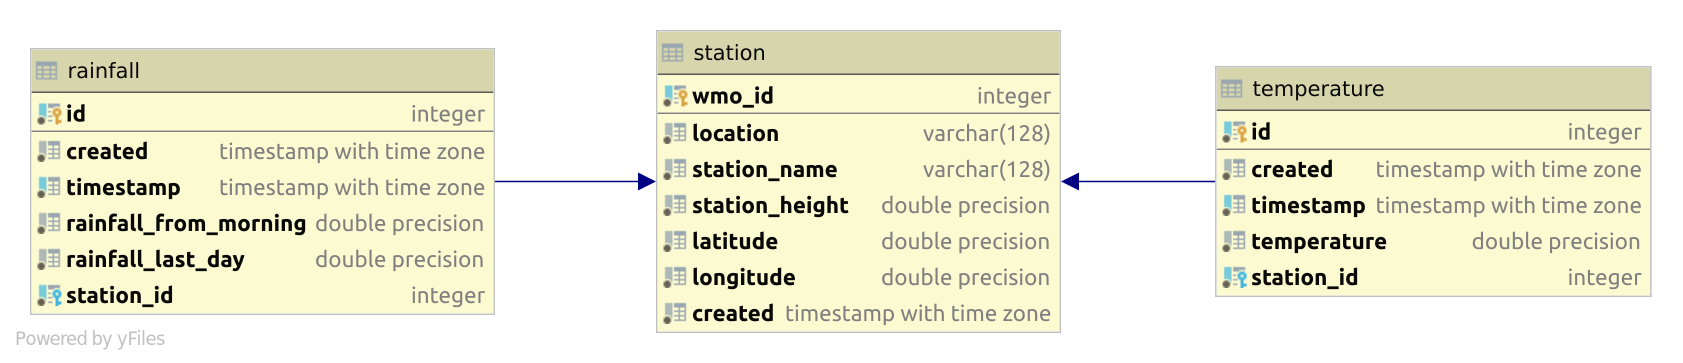
\includegraphics[width=.9\textwidth]{django-er-diagram.png}
        \caption{Databázové schéma pro uložení předpočítaných výsledků v~relační databázi}
    \end{figure}

    \subsection{computer}

    Výpočetní kontejner založený na jazyku Python s identifikátorem \texttt{computer} slouží ke spouštění agregačních
    dotazů nad nerelační databází v kontejneru \texttt{mongo}, zpracování výsledků a jejich následné uložení do databáze
    v kontejneru \texttt{postgres}.

    Podrobnější popis dotazů a jejich řešení pomocí agregací následuje:

    \subsubsection{Dotaz A}
    \emph{Vytvořte žebříček nejdeštivějších/nejsušších a nejteplejších/nejchladnějších meteorologických stanic/lokalit.}

    Získání dat v odpovídající struktuře a splňující podmínky prvního dotazu vychází z použití agregační \emph{pipeline}
    odeslané na kolekci \texttt{measurement} do databáze MongoDB. Každá část dotazu je realizována samostatnou
    agregací, avšak obě sdílí následující strukturu:
    \begin{itemize}
        \item \textbf{{\textdollar}match} -- do dalšího zpracování se vezmou pouze dokumenty, která jsou validní pro
        danou část dotazu (tedy obsahují teplotu vzduchu, resp. úhrny srážek)
        \item \textbf{{\textdollar}lookup} -- k datům měření se připojí data o stanici na základě klíče \texttt{station\_id}
        \item \textbf{{\textdollar}unwind} -- tento krok zajistí rozexpandování nalezených stanic k každému měření --
        vzhledem k povaze dat však ke každému měření odpovídá právě jedna stanice
        \item \textbf{{\textdollar}project} -- do dalšího zpracování jsou vzaty v potaz pouze některé
        atributy -- zejména samotná data identifikující měření (stanice, měsíc měření, čas měření) a také samotná
        hodnota měření
        \item \textbf{{\textdollar}sort} -- dokumenty jsou seřazeny dle stanice a času pořízení (pro snazší ladění)
        \item \textbf{{\textdollar}group} -- koncové seskupení do dávek měření, které odpovídající kompozitnímu klíči
        \texttt{[station\_id, timestamp]} a obsahují všechny měření z konkrétní stanice a času -- v
        samotných záznamech se poté již vyskytuje pouze změřená hodnota (resp. hodnoty) a konkrétní časový otisk
    \end{itemize}
    
    V případě nejdeštivějších/nejsušších míst byl problém s tím jak hledět na data, protože srážky jsou spojitá veličina a data obsahují počet srážek v čase od 9:00 do 9:00 následujícího dne v časovým pásmu stanice. Pro jednoduchost je čas měření počtu srážek brán jak koncový čas tohoto měření. 
    
    \subsubsection{Dotaz B}
    \emph{Najděte skupiny meteorologických stanic s~podobným počasím.}

    Před samotným řešením problému je vhodné lokálně definovat \emph{stanice s podobným počasím} -- pro účely tohoto
    dotazu mají dvě stanice podobné počasí, jestliže lze prokázat pozitivní korelaci mezi daty změřenými v těchto
    stanicích v odpovídajícím čase a zároveň v rámci stanovené odchylky odpovídají statistické metriky těchto
    měřených dat. Tedy pro příklad, pro konkrétní den odpovídá střední hodnota a směrodatná odchylka teplot vzduchu
    pro dvě \emph{stanice s podobným počasím} a zároveň je srovnatelný týdenní vývoj tohoto změřeného parametru.

    Možný SQL dotaz, který splňuje specifickou část požadavku je zobrazen v \ref{lst:sql-dotaz-b} a je založen na
    technice CTE implementované v použité databázi PostgreSQL. Jeho funkce je založena na vytvoření pomocné datové
    sady obsahující agregovaná data tak, že pro každou stanici a týden v roce je uložena standardní odchylka a
    střední hodnota teplot vzduchu v tom konkrétním týdnu. Takto připravená data jsou následně agregovaná dle obou
    statistických ukazatelů do množin dvojic $(\text{stanice}, \text{týden v roce})$, které již odpovídají
    \emph{stanicím s podobným počasím} -- aby došlo úspěšně ke generalizaci, jsou oba statistické ukazatele
    zaokrouhleny na celá čísla.

    Problém \emph{podobného počasí} lze přímo v modelové vrstvě řešit i mnohem sofistikovanějšími
    metodami, například pomocí n-dimenzionálního rozmístění stanic dle změřených příznaků a následného hledání 
    skupin stanic klasifikátorem \texttt{k-means} či jiného klasifikátoru určeného ke \emph{clusterizaci}. Takto
    fungující klasifikátor by mohl, dle znalostí autorů tohoto projektu, být založen na vlastní \texttt{window}
    funkci založené na technice CTE v rekurzivní variantě.

\begin{figure}[H]
    \begin{lstlisting}[language=SQL]
with measurements as (
    select
        s.wmo_id,
        extract(weeks from t.timestamp)                as week_number,
        ROUND(cast(stddev(temperature) as numeric), 0) as temperature_stddev,
        ROUND(cast(avg(temperature) as numeric), 0)    as temperature_avg
    from temperature t
        inner join station s on s.wmo_id = t.station_id
    where
        extract(year from t.timestamp) = 2020
    group by extract(weeks from t.timestamp), s.wmo_id
)
select
    m.temperature_avg,
    m.temperature_stddev,
    array_agg(cast(ARRAY [m.wmo_id, m.week_number] as int[2])) as stations_in_time
from measurements m
where
    temperature_stddev is not null and temperature_avg is not null
group by m.temperature_avg, m.temperature_stddev;
    \end{lstlisting}
    \caption{SQL dotaz pro nalezení \emph{stanic s podobným počasím} v konkrétních týdnech -- analogicky by vznikaly
    skupiny stanic na základě dalších parametrů \emph{počasí}.}
    \label{lst:sql-dotaz-b}
\end{figure}

    \subsection{superset}

    Tento kontejner slouží pro instanci nástroje Apache Superset, který je určen pro publikaci a vizualizaci
    zpracovaných dat uložených v databázi v kontejneru \texttt{postgres}. Jako pomocný kontejner pro cache slouží
    \texttt{redis} s instancí stejnojmenné databáze typu \texttt{key-value}.

    \section{Spuštění a práce s projektem}

    \subsection{Požadovaný software}\label{requirements}

    \begin{itemize}
        \itemsep1pt\parskip0pt\parsep0pt
        \item Docker engine 19.0 a vyšší
        \item Docker compose 1.25 a vyšší
    \end{itemize}

    \subsection{Inicializace služeb}\label{initialization-of-services}

    \begin{enumerate}
        \def\labelenumi{\arabic{enumi}.}
        \itemsep1pt\parskip0pt\parsep0pt
        \item Zapnutí potřebných kontejnerů:

        \begin{itemize}
            \itemsep1pt\parskip0pt\parsep0pt

            \item spuštění kontejnerů

            \begin{itemize}
                \itemsep1pt\parskip0pt\parsep0pt
                \item[] \texttt{\textdollar\ make up}
            \end{itemize}

            \item spuštění kontejnerů na pozadí

            \begin{itemize}
                \itemsep1pt\parskip0pt\parsep0pt
                \item[] \texttt{\textdollar\ make upd}
            \end{itemize}
        \end{itemize}

        \item Po spuštění příkazu je nutné vyčkat na nastartovanání služeb v kontejnerech a následně je možné
        inicializovat projekt následujícím příkazem (při běžíčících kontejnerech):

        \begin{itemize}
            \itemsep1pt\parskip0pt\parsep0pt
            \item[] \texttt{\textdollar\ make init}
        \end{itemize}

        \item A následně je možné načíst výchozí konfiguraci pro prezentační vrstvu:

        \begin{itemize}
            \itemsep1pt\parskip0pt\parsep0pt
            \item[] \texttt{\textdollar\ make restore-superset}
        \end{itemize}
    \end{enumerate}

    \subsection{Zastavení služeb}

    Pro zastavení služeb je možné použít příkaz \texttt{\textdollar\ make down}.

    \subsection{Správa dat}

    Pro přidání dat do NoSQL databáze je nutno v kořenu projektu vytvořit adresář \texttt{pocasi} a umístit do něj
    datovou sadu souborů určenou pro načtení -- to lze realizovat pomocí \texttt{\textdollar\ make scrape}.

    Následné spuštění výpočetní vrstvy je možné pomocí příkazu \texttt{\textdollar\ make compute}.

    \subsection{Správa uživatelů}

    Vytvoření uživatelů a administrátorů lze docílit dvěma způsoby -- buď v grafickém rozhraní Apache Superset nebo
    přes příkazovou řádku -- druhé pomocí \texttt{\textdollar\ make create-admin}, resp. \texttt{\textdollar\ make create-user}.

    \subsection{Porty služeb}
    \begin{longtable}[c]{@{}ll@{}}
        \toprule\addlinespace
        \textbf{Služba} & \textbf{Port}
        \\\addlinespace
        \midrule\endhead
        \href{http://localhost:8081}{mongo-admin} & 8081
        \\\addlinespace
        \href{http://localhost:8082}{postgres-admin} & 8082
        \\\addlinespace
        \href{http://localhost:8088}{superset} & 8088
        \\\addlinespace
        postgres & 5432
        \\\addlinespace
        mongo & 27017
        \\\addlinespace
        redis & 6379
        \\\addlinespace
        \bottomrule
    \end{longtable}
\end{document}
